% Created 2019-04-04 Thu 12:47
% Intended LaTeX compiler: pdflatex
\documentclass[presentation, smaller]{beamer}
\usepackage[utf8]{inputenc}
\usepackage[T1]{fontenc}
\usepackage{graphicx}
\usepackage{grffile}
\usepackage{longtable}
\usepackage{wrapfig}
\usepackage{rotating}
\usepackage[normalem]{ulem}
\usepackage{amsmath}
\usepackage{textcomp}
\usepackage{amssymb}
\usepackage{capt-of}
\usepackage{hyperref}
\usetheme{Frankfurt}
\usepackage{PTSans}
\usepackage[utf8]{inputenc}
\usepackage[T2A]{fontenc}
\usepackage[english, russian]{babel}
\usepackage{mathtools, amsmath, xspace}
\uselanguage{Russian}
\languagepath{Russian}
\newcommand{\dadi}{$\partial$a$\partial$i\xspace }
\setbeamertemplate{footline}{\insertpagenumber/\insertsectionendpage }
\setbeamertemplate{caption}[numbered]
\usepackage{slashbox}
\usetheme{default}
\author{Илья Шешуков \\ Руководители: Екатерина Носкова (ИТМО), \\ Вячеслав Боровицкий (СПбГУ)}
\date{}
\title{Байесовская оптимизация для вывода демографических историй}
\subtitle{Промежуточная презентация}
\hypersetup{
 pdfauthor={Илья Шешуков \\ Руководители: Екатерина Носкова (ИТМО), \\ Вячеслав Боровицкий (СПбГУ)},
 pdftitle={Байесовская оптимизация для вывода демографических историй},
 pdfkeywords={},
 pdfsubject={},
 pdfcreator={Emacs 26.1 (Org mode 9.2.1)}, 
 pdflang={English}}
\begin{document}

\maketitle

\begin{frame}[label={sec:org95f9b18}]{Введение}
\begin{block}{Демографическая модель популяции}
Имея геномы людей, хотим понять как изменялись их популяции.
Как менялась численность, когда популяции разделялись, как сильно они мигрировали.

\begin{figure}[htbp]
\centering
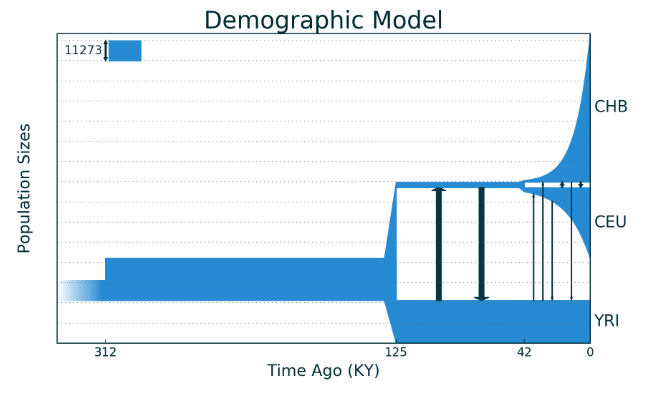
\includegraphics[width=2in]{./pics/outofafrica.png}
\caption{\label{fig:org8451681}
Популяционная модель человеческой миграции из Африки}
\end{figure}
\end{block}
\end{frame}

\begin{frame}[label={sec:org086f695}]{Аллель-частотный спектр}
\begin{definition}[Аллель-частотный спектр]
Аллель-частотный спектр это распределение частоты аллелей в данных локусах в
популяции или выборке.

\begin{figure}[htbp]
\centering
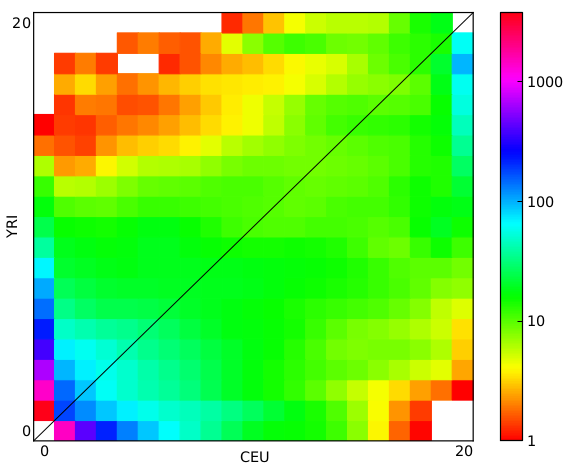
\includegraphics[width=2in]{./pics/sfs.png}
\caption{\label{fig:org22dc094}
Хитмэп аллель-частотного спектра двух популяций}
\end{figure}
\end{definition}
\end{frame}

\begin{frame}[label={sec:orgefff875}]{Пример}
\[
\begin{matrix}
  & SNP 1 & SNP 2 & SNP 3 & SNP 4 & SNP 5 & SNP 6 & SNP 7 & SNP 8 \\
\hline  & 0 & 1 & 0 & 0 & 0 & 0 & 1 & 0 \\
  & 1 & 0 & 1 & 0 & 0 & 0 & 1 & 0 \\
  & 0 & 1 & 1 & 0 & 0 & 1 & 0 & 0 \\
  & 0 & 0 & 0 & 0 & 1 & 0 & 1 & 1 \\
  & 0 & 0 & 1 & 0 & 0 & 0 & 1 & 0 \\
  & 0 & 0 & 0 & 1 & 0 & 1 & 1 & 0 \\
 \text{Сумма} & 1 & 2 & 3 & 1 & 1 & 2 & 5 & 1 \\
\end{matrix}
\]

Спектр: \(\begin{pmatrix}4&2&1&0&1\end{pmatrix}\)
\end{frame}

\begin{frame}[label={sec:orgef3d90b}]{Как это делается сейчас}
\begin{block}{\dadi}
\url{https://bitbucket.org/gutenkunstlab/dadi/}
\begin{itemize}
\item Плюсы
\begin{itemize}
\item Она работает
\item Ей пользуются реальные люди
\end{itemize}
\item Минусы
\begin{itemize}
\item Решает дифференциальное уравнение в частных производных, что долго
\item Использует методы локальной оптимизации, что малоэффективно
\item Для работы необходимо руками писать Питон
\end{itemize}
\end{itemize}
\end{block}

\begin{block}{moments}
\url{https://bitbucket.org/simongravel/moments}
\begin{itemize}
\item Плюсы
\begin{itemize}
\item Эффективнее, чем \dadi, особенно на больших популяциях
\end{itemize}
\end{itemize}
\end{block}
\end{frame}

\begin{frame}[label={sec:org5e0ee3f}]{GADMA}
\begin{block}{GADMA}
\url{https://github.com/ctlab/GADMA}
\begin{itemize}
\item Основана на \dadi и moments
\item Использует генетический алгоритм для поиска значения параметров
демографической модели
\item Не требует человеческого вмешательства
\end{itemize}
\end{block}
\end{frame}

\begin{frame}[label={sec:orgc61397a}]{Что можно сделать}
\begin{block}{Байесовская оптимизация}
\begin{itemize}
\item Хорошо работает для сложновычислимых функций (например, если нужно решать
уравнение в частных производных), т.е. хорошо подходит для задачи
\item Можно параллелить
\end{itemize}
\begin{center}
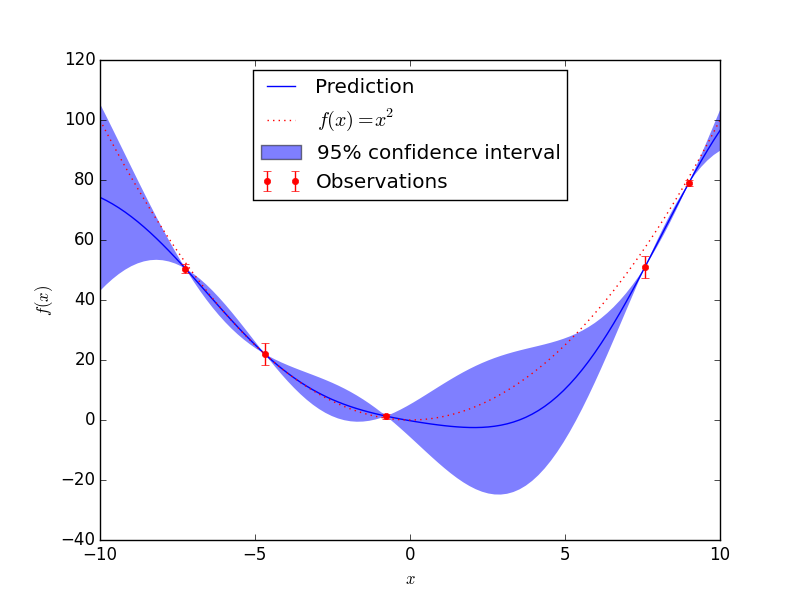
\includegraphics[width=2in]{./pics/bayes.png}
\end{center}
\end{block}
\end{frame}

\begin{frame}[label={sec:orgcfabea8}]{Планы}
\begin{enumerate}
\item (В процессе) Заменить в \dadi алгоритм градиентного спуска на байесовскую оптимизацию.
\item Посмотреть станет ли лучше
\item (Может быть?) Интегрировать в GADMA
\end{enumerate}
\end{frame}

\begin{frame}[label={sec:orga07d43a}]{Конец}
\begin{center}
Спасибо за внимание
\end{center}
\end{frame}
\end{document}
